\section{Mottos}\label{sec:mottos}

\begin{wrapfigure}{R}{0.3\textwidth}
\centering
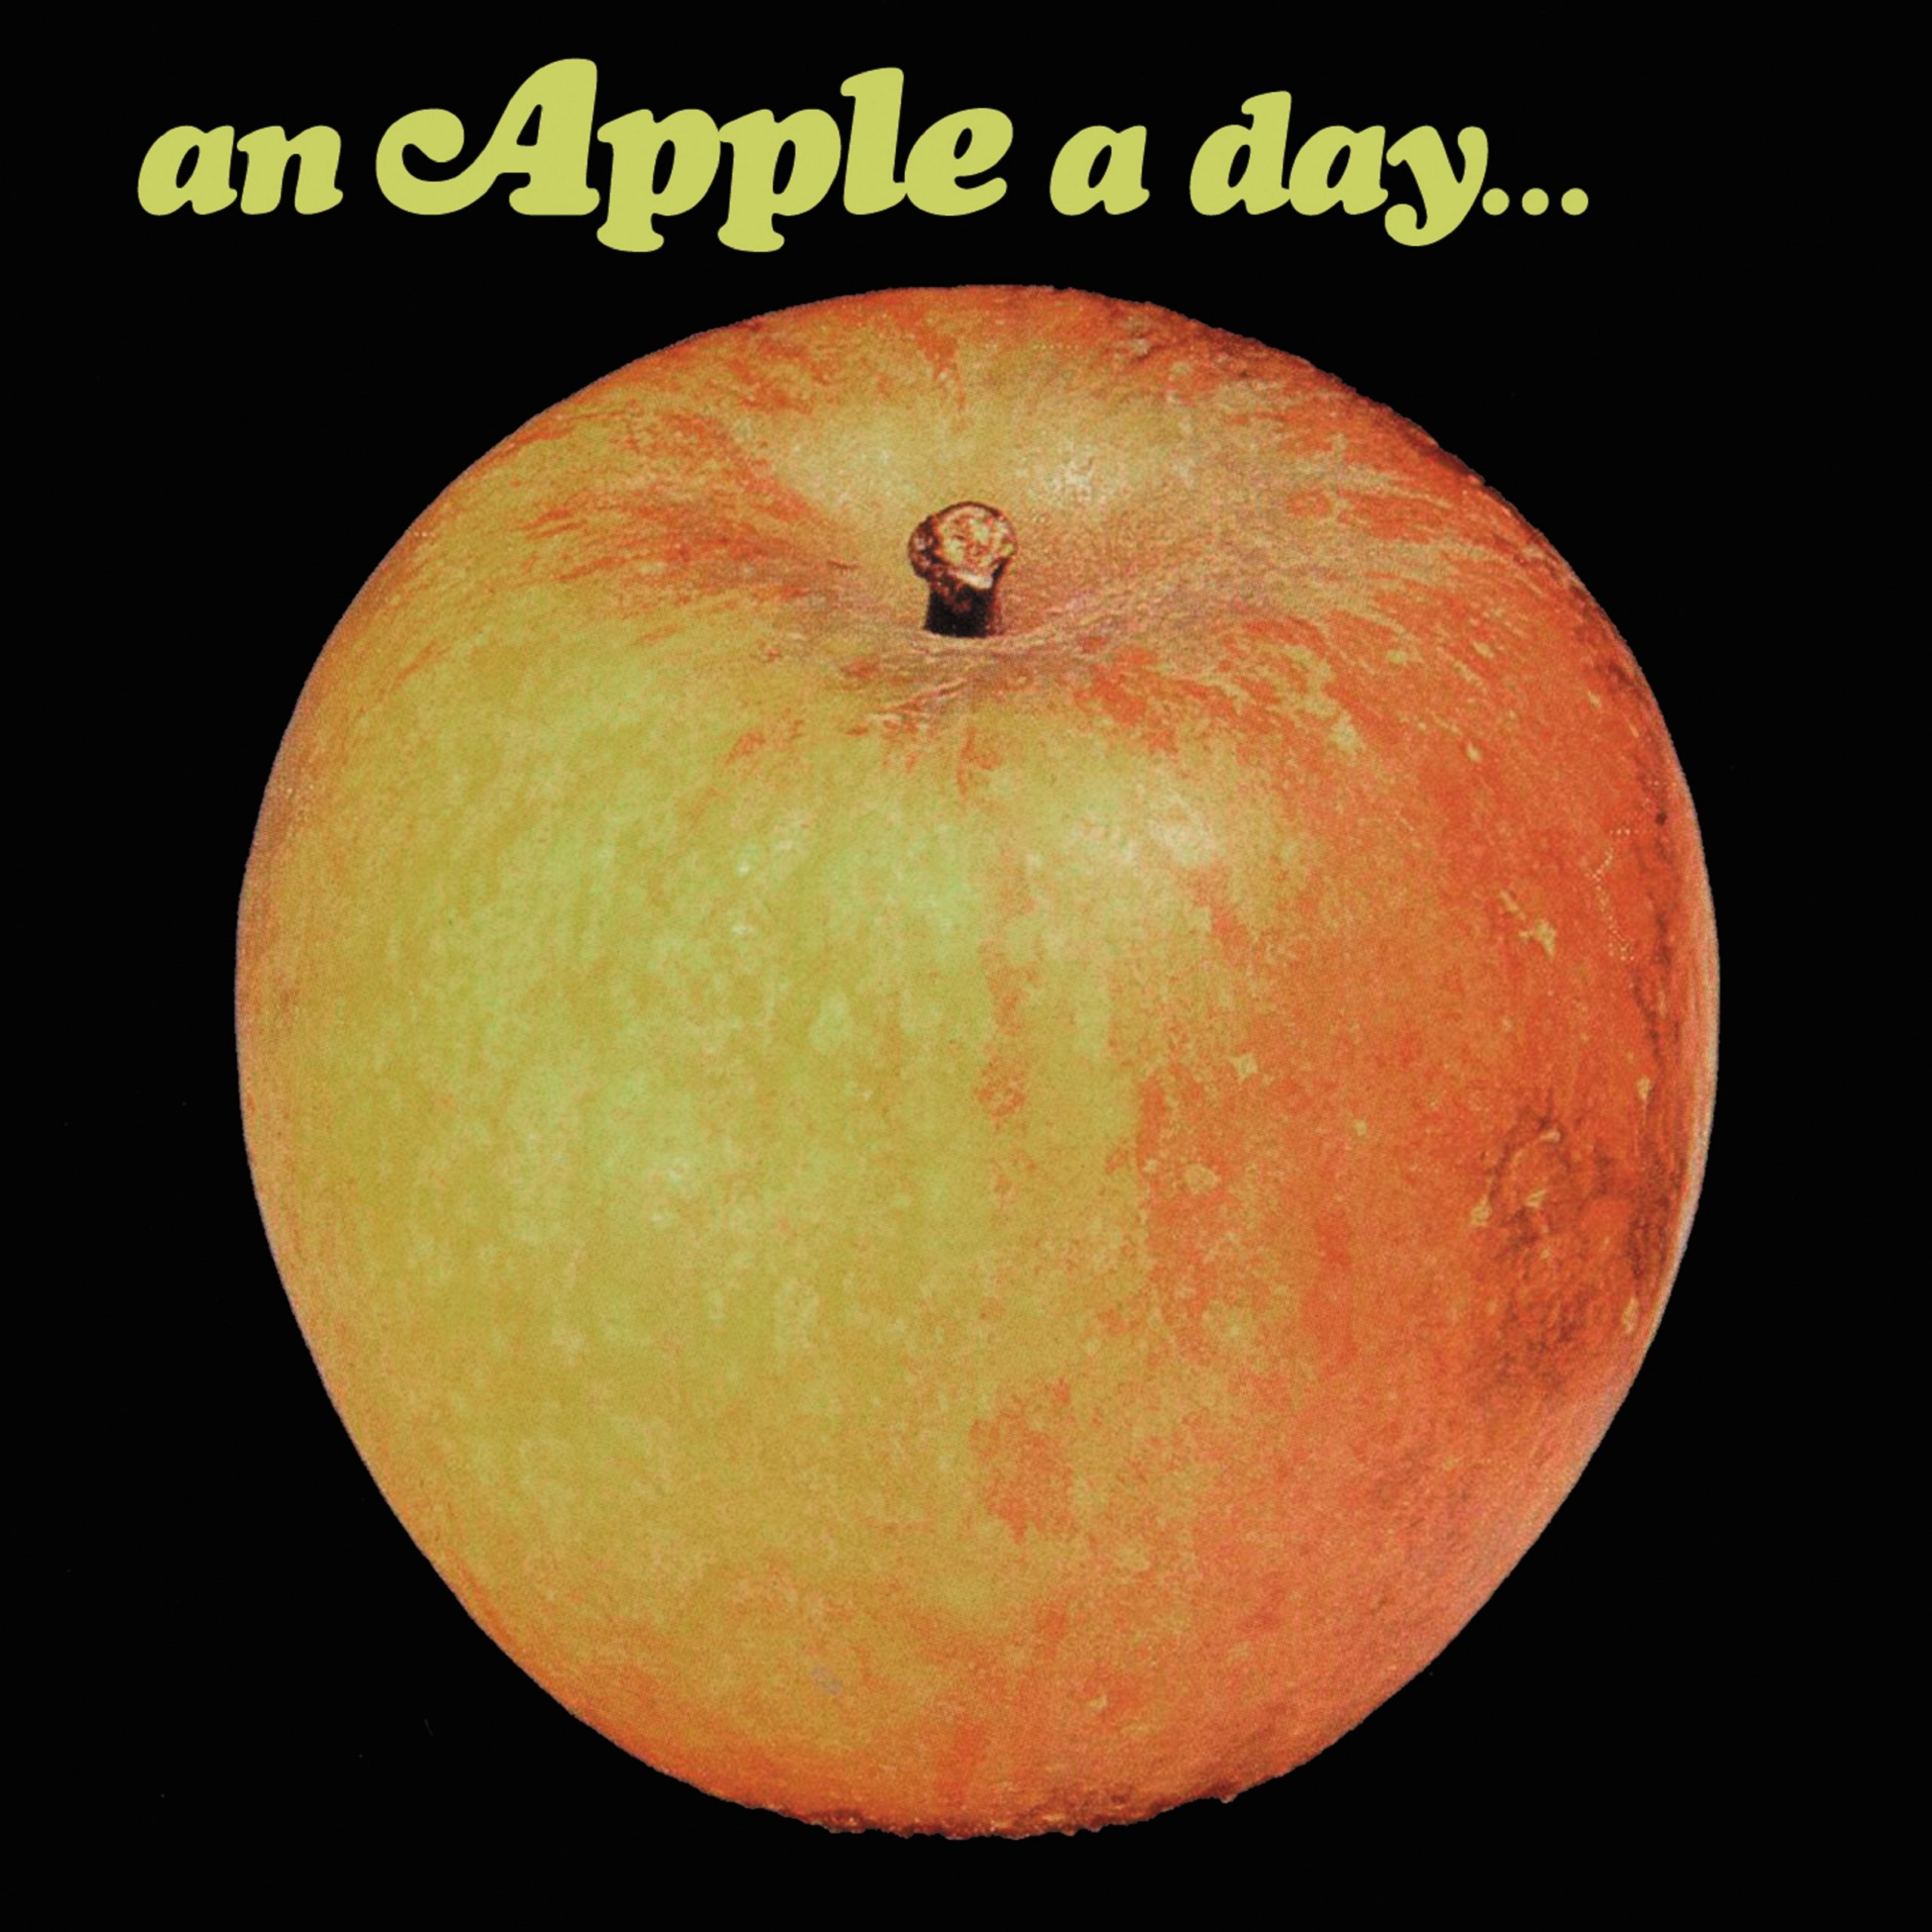
\includegraphics[width=0.25\textwidth]{images/mottos}
\end{wrapfigure}

You could also call them (universal) guidelines, which are semantically more specific than principles, yet not as specific as concrete techniques.
They help us improve our technique, implement the principles, and embody a CI quality.

For example:

\begin{itemize}
    \item \textit{Tension masks sensation.} Imagine your muscles are tensing up so much, they squeeze the nerves which then can't transmit any information anymore.
    The more relaxed we are, the more sensitive our skin is to touch and pressure/weight.
    \item \textit{Keep on breathing.} When getting tensed up, physically and emotionally, we humans tend to hold our breath, which is counterproductive to stay sharp, focused and relaxed.
    Instead, we continuously try to remind ourselves to breath, and especially emphasize a deep out-breath.
    \item \textit{Keep eyes open and ``wide''.} Sometimes people tend to close them, or focus them on the partner.
    Instead we want to keep an open gaze, perceiving everything around us, staying in connection with all the people in the room and the room itself.
    Once we start to gaze at the floor, this is usually an indication of a hyper-focus which potentially closes our perception.
\end{itemize}
